\documentclass[usenatbib,usegraphicx,letterpaper]{mn2e}
\usepackage[totalwidth=480pt,totalheight=680pt]{geometry}

\usepackage{amssymb}
\usepackage{epsfig}
\usepackage{amsmath}
\usepackage{color}

\bibliographystyle{mn2e}

%-------- journals
\newcommand{\araa}{ARAA~}
\newcommand{\apj}{ApJ~}
\newcommand{\apjl}{ApJL~}
\newcommand{\apjs}{ApJS~}
\newcommand{\mnras}{MNRAS~}
\newcommand{\nat}{Nature~}
\newcommand{\physrep}{Phys. Rep.~}
\newcommand{\aj}{AJ~}
\newcommand{\pasp}{ASP~}

%%%% Misc %%%
\newcommand{\beq}{\begin{equation}}
\newcommand{\eeq}{\end{equation}}
\newcommand{\beqray}{\begin{eqnarray}}
\newcommand{\eeqray}{\end{eqnarray}}

\newcommand{\ben}{\begin{enumerate}}
\newcommand{\een}{\end{enumerate}}
\newcommand{\bit}{\begin{itemize}}
\newcommand{\eit}{\end{itemize}}

%%%%%%%%  galaxy properties  %%%%%%%%
\newcommand{\rhalf}{R_{1/2}}
\newcommand{\rhalfdisk}{R_{1/2}^{\rm disk}}
\newcommand{\rhalfbulge}{R_{1/2}^{\rm bulge}}
\newcommand{\adisk}{A_{\rm disk}}
\newcommand{\abulge}{A_{\rm bulge}}
\newcommand{\alphadisk}{\alpha_{\rm disk}}
\newcommand{\alphabulge}{\alpha_{\rm bulge}}
\newcommand{\sigmarhalf}{\sigma_{\rm R_{1/2}}}
\newcommand{\rvir}{R_{\rm vir}}
\newcommand{\bt}{{\rm B/T}}
\newcommand{\mstar}{M_{\ast}}
\newcommand{\ssfr}{{\rm sSFR}}
\newcommand{\sfr}{{\rm SFR}}

%%%%%%%%  halo properties  %%%%%%%%
\newcommand{\halospin}{\lambda_{\rm halo}}
\newcommand{\mvir}{M_{\rm vir}}
\newcommand{\macc}{M_{\rm acc}}
\newcommand{\mpeak}{M_{\rm peak}}
\newcommand{\mhalo}{M_{\rm halo}}


%%%%%%%%  observations  %%%%%%%%
\newcommand{\rproj}{r_{\rm p}}
\newcommand{\wproj}{w_{\rm p}}

%%%%%%%%  units  %%%%%%%%
\newcommand{\kpc}{{\rm kpc}}
\newcommand{\mpc}{{\rm Mpc}}
\newcommand{\msun}{M_\odot}
\newcommand{\kms}{{\rm km/s}}

%%%%%%%%%%%%%%%%%%%%%%%%%%%%%%%%
%%%%%%%%%%%%%%%%%%%%%%%%%%%%%%%%


\usepackage{epsfig}  \usepackage{graphicx}   \usepackage{rotating}

\begin{document}

\title[The Emergent Simplicity of Galaxy Size]
{The Emergent Simplicity of Galaxy Size}


\author[Hearin, Behroozi, Kravtsov \& Moster]{
Andrew Hearin$^{1}$, Peter Behroozi$^{2}$, Andrey Kravtsov$^{3}$, Benjamin Moster$^{4}$\\
$^{1}$Argonne National Laboratory, Argonne, IL, USA 60439, USA\\
$^{2}$Department of Physics, University of Arizona, 1118 E 4th St, Tucson, AZ 85721 USA\\
$^{3}$Department of Astronomy \& Astrophysics, The University of Chicago, Chicago, IL 60637 USA\\
$^{4}$Universit{\"a}ts-Sternwarte, Ludwig-Maximilians-Universit{\"a}t M{\"u}nchen, Scheinerstr. 1, 81679 M{\"u}nchen, Germany
}

\maketitle

\begin{abstract}
We derive empirical modeling constraints on the connection between dark matter halos and the half-light radius $\rhalf$ of galaxies. Using forward-modeling techniques based on {\tt Halotools}, we confirm previous results in Kravtsov (2013) that $\rhalf$ is well-described by a linear scaling relation with halo virial radius. Novel to this work, we use new SDSS measurements of the $\rhalf-$dependence of galaxy clustering to test this modeling assumption. With no changes to the parameters, the model accurately predicts the observed two-point clustering on small- and large-scales over a wide range of stellar mass. This quantitative success is remarkable since the Kravtsov (2013) parameters were fit to the observed $\langle\rhalf\vert\mstar\rangle,$ and the $\rhalf-$dependence of SDSS galaxy clustering has heretofore never been measured. Moreover, this success is non-trivial, as we demonstrate that galaxy clustering is highly sensitive to the assembly history-dependent physics that shapes the relative size of centrals and satellites. Our results can be treated as a boundary condition for more complex and fine-grained models of galaxy size, and provide a simple means for cosmological surveys to generate synthetic galaxy populations with realistic sizes across the cosmic web.
\end{abstract}

\section{Introduction}
\label{sec:intro}
Some introduction goes here.

\section{Data and Simulations}
\label{sec:data}

Our galaxy sample comes from the catalog of SDSS galaxy profile decompositions provided by \citet{meert_etal15}. This catalog is based on Data Release 10 of the Sloan Digital Sky Survey \citep[SDSS,][]{ahn_etal14}, with improvements to the photometry pipeline and light profile fitting methods \citep{vikram_etal10,bernardi_etal13,bernardi_etal14,meert_etal13}. In the version of this catalog that we use, two-dimensional $r-$band profiles were fit with a two-component de Vaucouleurs + exponential profile to determine the half-light radius $\rhalf.$ We apply the \citet{bell_etal03} mass-to-light ratio to the $r-$band flux and $g-r$ colors in this catalog to obtain an estimate for the total stellar mass $\mstar$ of every galaxy.

We calculate two-point clustering $\wproj$ of our SDSS galaxy sample using line-of-sight projection of $\pi_{\rm max}=20\mpc$ using the {\tt correl} program in {\tt UniverseMachine}. Our results in \S~\ref{sec:results} will give special focus on the dependence of $\wproj$ upon $\rhalf.$ We will quantify this dependence in terms of {\em clustering ratios} of ``large" vs. ``small" galaxies, defined according to whether composite galaxy size is above or below $\langle\rhalf\vert\mstar\rangle,$ computed as the median of a sliding stellar mass window with a width of $N_{\rm gal}=1000.$

As the bedrock of our modeling, we use the catalog of {\tt Rockstar} subhalos identified at $z=0$ in the Bolshoi-Planck simulation \citep{klypin_etal11,behroozi12_rockstar,behroozi12_consistent_trees,riebe_etal13,rodriguez_puebla16_bolplanck}. the particular version of the catalog we use is made publicly available through {\tt Halotools} \citep{hearin_etal16}, with {\tt version\_name} = `halotools\_v0p4'. For mock galaxies, to compute galaxy clustering we employ the distant observer approximation by treating the simulation $z-$axis as the line-of-sight. We compute $\wproj$ using the {\tt mock\_observables.wp} function in {\tt Halotools}, which is a python implementation of the algorithm in the {\tt Corrfunc} C library \citep{sinha_etal17}. 

All numerical values of $\rhalf$ will be quoted in $\kpc,$ and all values of $\mstar$ and $\mhalo$ in $\msun,$ assuming $H_0=67.8~\kms\equiv100h~\kms,$ the best-fit value from \citet{planck15}. To scale stellar masses to ``$h=1$ units" \citep{croton13}, our numerically quoted values for $\mstar$ should be multiplied by a factor of $h^2,$ while our halo masses and distances should be multiplied by a factor of $h.$


\section{Galaxy-Halo Model}
\label{sec:model}

Motivated by the \citet{kravtsov13} results, we model the half-mass radii of galaxies as separate power law functions of halo virial radius:

\begin{eqnarray}
\label{eq:fiducial_model}
\rhalfbulge &=& \abulge\rvir^{\alphabulge} \\
\rhalfdisk &=& \adisk\rvir^{\alphadisk}
\end{eqnarray}

For central galaxies residing in host halos, we use the present-day virial radius; for satellite galaxies we use the virial radius at the time of accretion, using physical units of $\kpc.$ We model the composite size of model galaxies as
\beq
\rhalf = (\bt)\rhalfbulge + (1-\bt)\rhalfdisk.
\eeq

When generating Monte Carlo realizations of our model galaxy population, we add log-normal scatter $\sigmarhalf$ separately to each component. Our model for sizes thus has five free parameters: $\abulge, \adisk, \alphabulge, \alphadisk,$ and $\sigmarhalf.$

We reiterate an important distinction drawn in the formulation of our forward modeling approach. In the model described above, $\rhalfbulge$ and $\rhalfdisk$ are forward modeling quantities that we aim to constrain through SDSS observations of {\em composite} galaxy size $\rhalf.$ In particular, both model and real galaxies will be categorized as ``small" or ``large`` according to whether $\rhalf$ is above or below the median size for a galaxy with total stellar mass $\mstar.$

\section{Results}
\label{sec:results}

In \S~\ref{subsec:tests1} we show comparisons between the fiducial galaxy profile model described in \S~\ref{sec:model} and our SDSS sample. We demonstrate the sensitivity of galaxy clustering measurements to the post-infall evolution of satellite profiles in \S~\ref{subsec:tests2}, establishing the success of our fiducial model as non-trivial. In \S~\ref{subsec:tests3} we show that even highly idealized measurements of galaxy clustering and lensing are insensitive to assumptions about the relation between halo spin $\halospin$ and size $\rhalf$ of disk-dominated galaxies, implying that large-scale structure observations yield little-to-no constraining power on such assumptions.

\subsection{Tests of the Fiducial Power Law Model}
\label{subsec:tests1}

\subsubsection{Scaling of $\rhalf$ with $\mstar$}
\label{subsubsec:scaling_relation}

In Figure \ref{fig:scatter_plot} we show the scaling of composite galaxy size $\rhalf$ with $\mstar,$ with separate panels dedicated to subsamples of galaxies divided according to value of $\bt.$ We refer to galaxies with $\bt<0.25$ as ``disk-dominated", $\bt>=0.75$ as ``bulge-dominated", and $0.25<=\bt<0.75$ as ``mixed morphology". We remind the reader that $\rhalf$ and $\mstar$ refer to the scale radius and stellar mass of the {\em entire} galaxy, not of an individual component.

%---------------------------------------------------------------------------------------------------
\begin{figure}
\centering
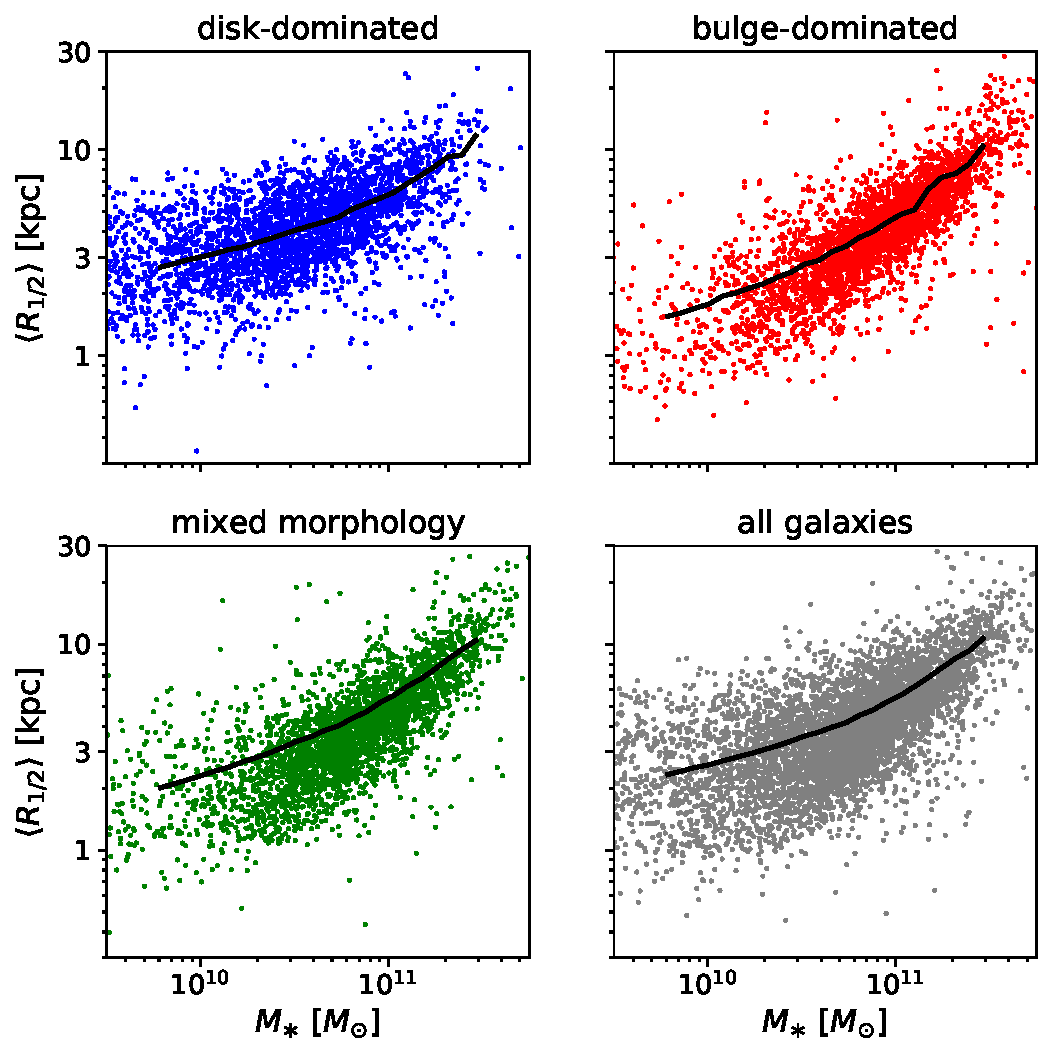
\includegraphics[width=8cm]{FIGS/size_vs_stellar_mass_multipanel_bt_decomposition.pdf}
\caption{
{\bf One-point data used to fit the fiducial model.}
Scattered points show the $\rhalf-\mstar$ relation for SDSS galaxies as measured in \citet{meert_etal15}. Bulge-dominated galaxies are defined in terms of the bulge-to-total stellar mass ratio $\bt>=0.75,$ disk-dominated galaxies $\bt<0.25,$ mixed morphology as $0.25 < \bt < 0.75.$ The black curve in each panel shows the $\rhalf-\mstar$ relation implied by our fiducial model, in which $\rhalfbulge=\abulge\rvir^{\alphabulge}$ and $\rhalfdisk=\adisk\rvir^{\alphadisk},$ with $\adisk=0.014=7\abulge, \alphadisk=1, \alphabulge=5/4,$ and uncorrelated log-normal scatter of $0.2$ dex about these relations.
}
\label{fig:scatter_plot}
\end{figure}
%-----------------------------------------------------------------------------------------------------

The results shown in \citet{kravtsov13} simplify our task of parameter space exploration: the assumption that composite galaxy size $\rhalf$ scales in linear proportion to halo radius $\rvir$ gives a qualitatively good description of SDSS data over many orders of magnitude in galaxy mass. As first pointed out in \citet{kravtsov13}, this linearization is non-trivial because of the well-known curvature in the scaling relation of $\langle\rhalf\vert\mstar\rangle,$ which is visually apparent in all panels of Fig.~\ref{fig:scatter_plot}.

Comparison of the top panels of Fig.~\ref{fig:scatter_plot} show that this linearization is only approximate; evidently, galaxy size $\rhalf$ of bulge-dominated systems has a steeper scaling relation with $\mstar$ relative to disk-dominated systems. This difference motivates our simple extension of the \citet{kravtsov13} model, in which $\rhalf$ of disk- and bulge-dominated galaxies scales according to separate power laws.

Through MCMC parameter space exploration aided by {\tt emcee} \citep{emcee_hammer}, we find a good description of the observed one-point scaling relations is given by model galaxies with the parameters $\adisk=0.014=7\abulge, \alphadisk=1, \alphabulge=5/4,$ with log-normal scatter of $0.2$ dex motivated by \citet{somerville_etal17}. The black curves in Fig.~\ref{fig:scatter_plot} illustrate the median $\langle\rhalf\vert\mstar\rangle.$

We confirm the visual impression of comparing the top panels of Fig.~\ref{fig:scatter_plot}: we are unable to find a parameter combination in which the composite size of both bulge- and disk-dominated galaxies have linear ($\alpha=1$) scaling with $\rvir.$ We do not quantitatively rule out such a scaling relation, as this would require careful investigation of the systematic error budget of galaxy profile modeling that we consider beyond the scope, though well-motivated, by the present work.

\subsubsection{Dependence of clustering on $\rhalf$}
\label{subsubsec:clustering_tests}

In this section we present new measurements of the $\rhalf-$dependence of projected galaxy clustering, $\wproj(\rproj).$ Galaxy clustering has complex, simultaneous dependence upon $\mstar,$ $\ssfr,$ $\rhalf,$ and $\bt.$ Since the purpose of this work is to test models of composite galaxy size $\rhalf,$ we design a measurement that is specifically tailored to isolate the influence of $\rhalf$ on the two-point function, while minimizing the dependence upon the other correlated variables.

To achieve this, we compute projected clustering separately for $\mstar-$complete samples of galaxies defined by simultaneous cuts on $\bt$ and $\rhalf,$ described as follows. First, we construct subsamples of disk-dominated and bulge-dominated galaxies using cuts of $\bt<0.25$ and $\bt>0.75,$ respectively, as in \S~\ref{subsubsec:scaling_relation} above. Separately for each $\bt-$selected subsample, we calculate $\langle\rhalf\vert\mstar;\bt\rangle,$ the median composite size of the sample as a function of total galaxy stellar mass. We split each $\bt-$selected sample in half according to whether the galaxy has a size $\rhalf$ that is above or below this median value. For any $\mstar-$complete threshold, this gives four subsamples of large and small, disk- and bulge-dominated galaxies. For each $\bt-$selected sample, we calculate the difference $\wproj^{\rm large}-\wproj^{\rm small},$ scaled by $\wproj^{\rm all},$ the clustering of the $\bt-$selected sample prior to splitting on $\rhalf,$ and refer to this quantity as {\em the $\rhalf$ clustering ratio}.

%---------------------------------------------------------------------------------------------------
\begin{figure}
\centering
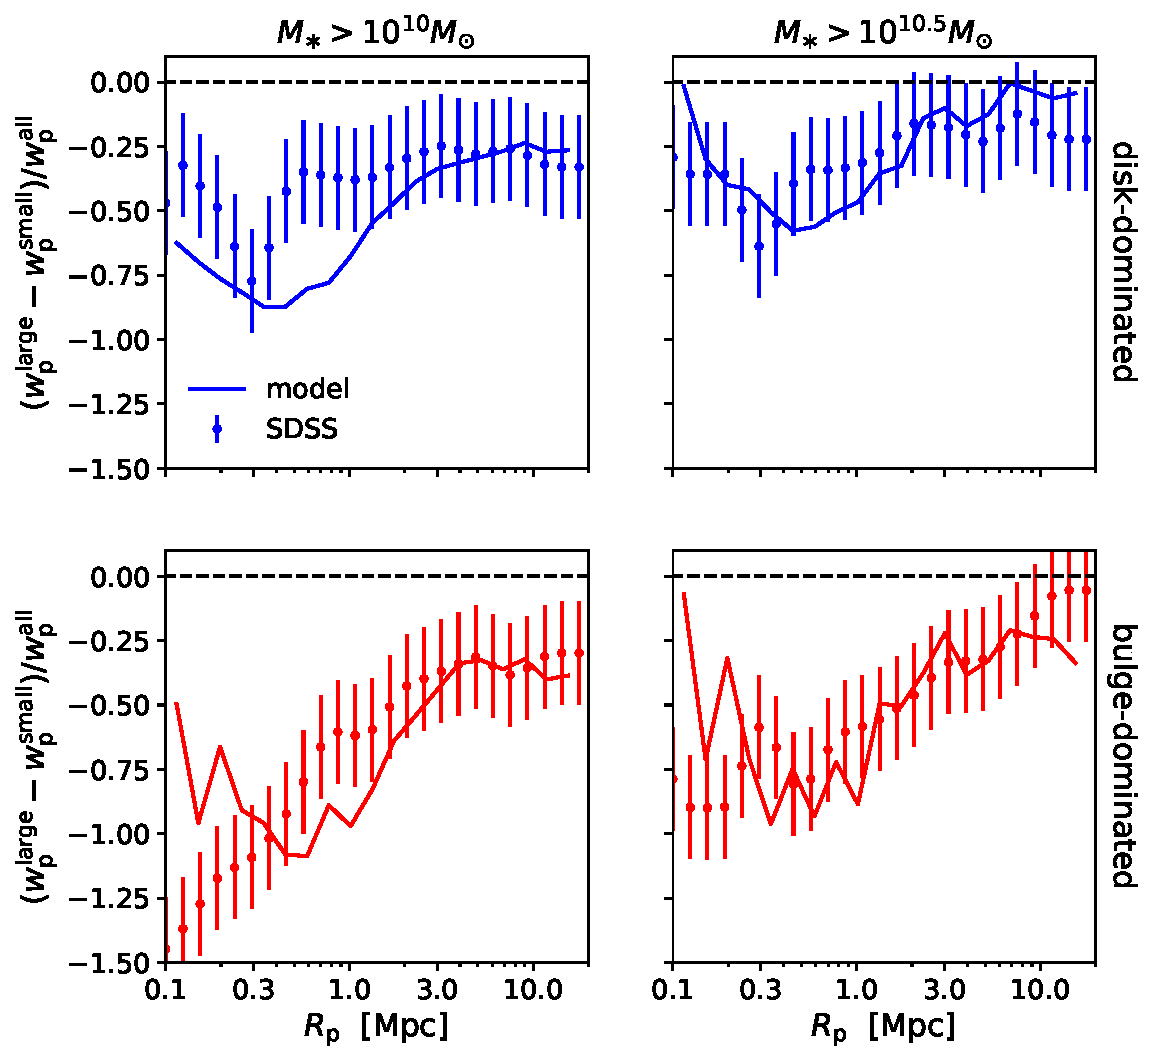
\includegraphics[width=8cm]{FIGS/size_clustering_ratios_bt_decomposition_model_vs_sdss.pdf}
\caption{
{\bf Two-point clustering predictions of the fiducial model.}
Points with error bars show new SDSS measurements of the $\rhalf-$dependence of projected galaxy clustering, $\wproj,$ compared to predictions by the model tuned to the measurements shown in Fig.~\ref{fig:scatter_plot}. We define a disk or bulge as ``large" or ``small" according to whether it is above or below the median size for its stellar mass. The y-axis shows clustering strength ratios, so that, for example, a y-axis value of $-0.5$ corresponds to small galaxies being $50\%$ more strongly clustered than large galaxies of comparable stellar mass. We show results separately for disk-dominated galaxies ({\em top} panels) and bulge-dominated galaxies ({\em bottom }panels), and different thresholds in total stellar mass in the {\em left} and {\em right} panels. The successful prediction shown here is remarkable because the model was not fit to these data, and because two-point clustering is highly sensitive to the physics that shapes satellite galaxy profiles (see Fig.~\ref{fig:satellites}).
}
\label{fig:clustering_ratio_upshot}
\end{figure}
%-----------------------------------------------------------------------------------------------------


The y-axis of each panel in Figure \ref{fig:clustering_ratio_upshot} shows these $\rhalf$ clustering ratios, with left and right panels showing measurements for $\mstar>10^{10}M_{\odot}$ and $\mstar>10^{10.5}M_{\odot}$ thresholds in total stellar mass, and top and bottom panels showing results for disk- and bulge-dominated samples, respectively. Points with error bars show SDSS measurements, solid curves show the clustering ratios of model galaxies. Before unpacking the information contained in these clustering measurements, we stress that the good agreement shown between model and data in Figure~\ref{fig:clustering_ratio_upshot} is a genuine model prediction, since we only tuned parameters to fit the one-point measurements in Fig.~\ref{fig:scatter_plot}.

The salient feature of the clustering ratio measurements is that they are negative: for either disk- or bulge-dominated samples, small galaxies cluster more strongly than large galaxies of the same stellar mass threshold, a new result. This feature also holds true for model galaxies, for which both $\rhalfbulge$ and $\rhalfdisk$ scale in power law proportion to $\rvir.$ Since halo mass $\mvir\propto\rvir^{3},$ and clustering is a strong function of $\mvir,$ the result may seem surprising.

The resolution to this puzzle is illustrated in Figure~\ref{fig:bt_censat}, which shows the PDF of $\bt$ for halos of the same mass $\mhalo,$ defined as $\mpeak,$ the peak mass ever attained through the history of the (sub)halo, so that host halos and subhalos can be treated on equal footing. In the model, central galaxies are diskier than satellites, a feature that is inherited from the method we use to map $\bt$ to model galaxies.

%---------------------------------------------------------------------------------------------------
\begin{figure}
\centering
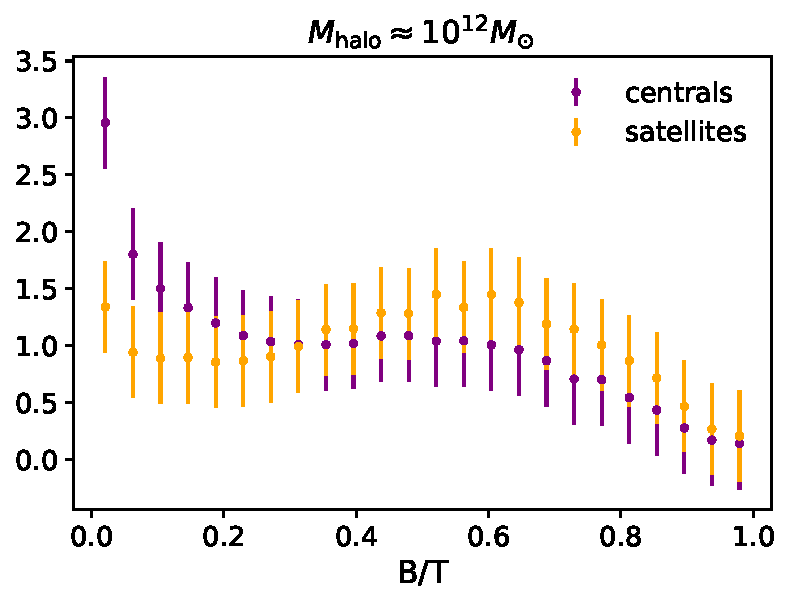
\includegraphics[width=8cm]{FIGS/random_bt_centrals_vs_satellites.pdf}
\caption{
{\bf Morphologies of centrals and satellites of the same halo mass.} We show the PDF of the bulge-to-total stellar mass ratio $\bt$ of central and satellite galaxies of the same halo mass $\mhalo=\mpeak.$ In the model, the PDF of $\bt$ is determined by the stellar mass $\mstar$ and specific star-formation rate $\ssfr$ statistically determine, with no residual dependence on the cosmic web. Satellite galaxies in the model are ``bulgier" than centrals of the same halo mass because satellites are more quiescent than centrals of the same stellar mass. Thus our baseline model ansatz is that the morphology-density relation is purely derived from the color-density relation. Since composite size $\rhalf$ in the model is given by $\rhalf\equiv\rhalf=(\bt)\rhalfbulge + (1-\bt)\rhalfdisk,$ this ansatz in turn implies that smaller galaxies cluster more strongly relative to larger galaxies of the same stellar mass, as seen in the measurements shown in Fig.~\ref{fig:clustering_ratio_upshot}.
}
\label{fig:bt_censat}
\end{figure}
%-----------------------------------------------------------------------------------------------------

In the {\tt UniverseMachine}, and in any quantitatively successful cosmological model of galaxy formation, central galaxies are preferentially more star-forming relative to satellites of comparable stellar or halo mass. Since bluer galaxies are diskier than redder galaxies, our model centrals will be diskier than satellites. Our galaxy profile model has $\adisk=7\abulge,$ and so satellite galaxies will be smaller than centrals due to the $\bt-\ssfr$ correlation. These simultaneous features alone will naturally result in the negative sign of the clustering ratios seen in Figure~\ref{fig:clustering_ratio_upshot}.

In light of this explanation, it is natural to ask whether this simple feature {\em alone} is all that is needed for any model of $\rhalf$ to achieve this level of success at predicting galaxy clustering on small and large scales. We address this question in \S~\ref{subsec:tests2} below, finding that the answer is no: the reasonably correct magnitude and scale-dependence of the clustering ratios predicted by our model is a non-trivial result that places tight constraints on the post-infall physics of satellite galaxies.

\subsection{Sensitivity of Clustering to Satellite Profile Evolution}
\label{subsec:tests2}

In this section we explore how post-infall changes in satellite $\rhalf$ manifest in $\wproj(\rproj).$ To do so, we construct an extension our fiducial model with a simple additional ingredient for post-infall size evolution of satellites.

In the fiducial model described in \S~\ref{sec:model}, recall that in the power law a scaling relations (Eq.~\ref{eq:fiducial_model}) the halo radius $\rvir$ used for satellite galaxies is taken to be the value at the time of infall. The simple interpretation of this assumption is that, in a statistical sense, the size of satellite galaxies is determined by its history as a central galaxy, and that post-infall physics leaves no distinct imprint on satellite $\rhalf.$

Here we suppose that this assumption is violated, and that $\rhalf$ decreases after infall according to $(\mvir/\macc)^{1/3}.$ That is, in this alternative formulation, rather than using $\rvir$ at the time of infall for satellites in the power law scaling relations, we instead use $\rvir(\mvir/\macc)^{1/3}.$ This simple toy model attempts supposes that the same physical processes leading to halo mass loss are also responsible for a post-infall decrease in satellite size.

%---------------------------------------------------------------------------------------------------
\begin{figure}
\centering
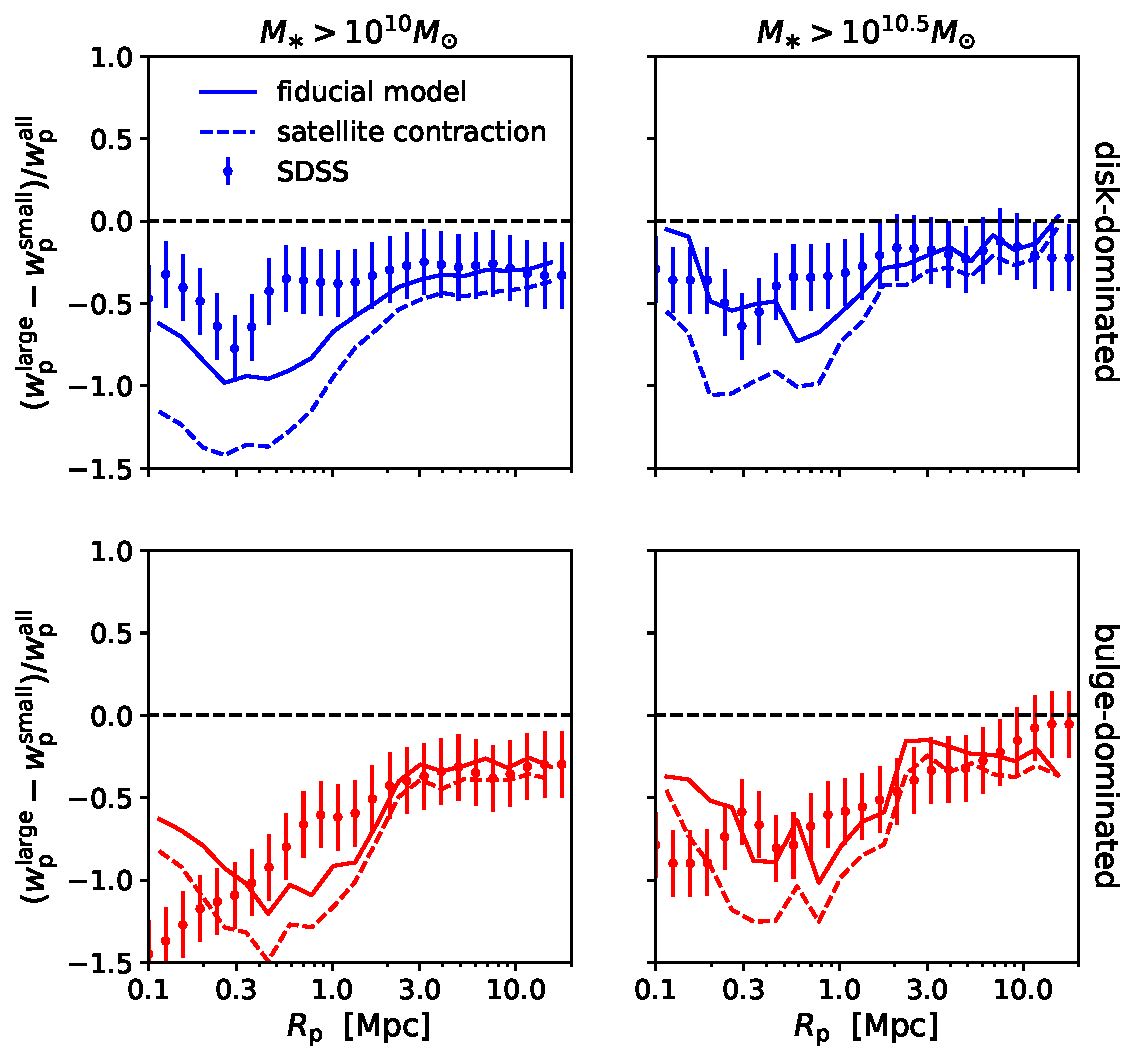
\includegraphics[width=8cm]{FIGS/alternate_satellite_models_size_clustering_ratios.pdf}
\caption{
{\bf Clustering tightly constrains satellite-specific size evolution.}
Here we compare our fiducial model, in which satellite galaxy size is set by $\rvir$ at the time of infall, to an alternative model analogous to \citet{watson_etal12} in which satellite sizes contract in proportion to $(\mvir/\macc)^{1/3}.$ The large differences between solid and dashed curves in the top panels show that the $\rhalf-$dependence of galaxy clustering ratios is highly sensitive to the post-infall evolution of satellite galaxy profiles. The successful prediction of our fiducial model, in which satellite galaxies neither contract nor puff up after infall, places tight constraints on satellite-specific physical processes, which must be either negligible or conspiratorially produce little-to-no size change after accretion.
}
\label{fig:satellites}
\end{figure}
%-----------------------------------------------------------------------------------------------------

Figure~\ref{fig:satellites} compares the clustering ratios of our fiducial model (solid curves) to the clustering ratios of this alternative model (dashed curves). The difference between the small-scale clustering of the two models is stark: the assumption that $\rhalf$ decreases after infall leaves a strong imprint on the $\rhalf-$dependence of $\wproj(\rproj),$ such that small galaxies cluster {\em much} more strongly relative to large galaxies, particularly for disk-dominated systems with $\mstar\approx10^{10}\msun.$

The large differences between the solid and dashed curves in Fig.~\ref{fig:satellites} establishes that the largely successful prediction for the clustering ratios fiducial model is a non-trivial: $\wproj(\rproj)$ is indeed providing good constraining power on the  assumptions underlying our profile modeling and not simply our morphology modeling, c.f., \S\ref{subsubsec:random_bt_model} and \S\ref{sec:model}. We refer the reader to \S\ref{subsec:satellite_discussion} for further discussion of the physical implications of this result.

\subsection{Insensitivity of Clustering and Lensing to Halo Spin Correlations}
\label{subsec:tests3}

The results of the previous section \S\ref{subsec:tests2} illustrate the sensitive constraints that galaxy clustering measurements provide on modeling assumptions about satellite $\rhalf.$ In this section we explore the potential constraining power of clustering on models for the size of disks of central galaxies. In particular, we seek to assess whether clustering measurements can constrain the long-standing assumption that disk size scales in proportion to the spin of the parent halo, $\rhalfdisk\propto\halospin,$ \citep[e.g.,][]{mo_mao_white98}.

We wish to build an alternative empirical model that inherits the quantitative success of our fiducial model, and further makes the extreme assumption that central galaxy $\rhalfdisk$ is maximally correlated with $\halospin$ at fixed $\mstar.$ Conditional Abundance Matching \citep[hereafter, CAM,][]{hearin_etal13b} is the natural framework to use to build such a model.

Disk size in our fiducial model has log-normal scatter $\sigmarhalf=0.2$ dex about the mean value $\adisk\rvir^{\alphadisk}.$  We use the CAM implementation in {\tt Halotools}\footnote{See {\tt halotools.empirical\_models.conditional\_abunmatch} documentation for details.} to extend our fiducial model so that the scatter in central galaxy $\rhalfdisk$ is not stochastic, but is in stead in one-to-one correspondence with $\halospin$ at fixed total stellar mass $\mstar.$ This alternative model thus has exactly the same one-point functions as the fiducial model (i.e., the solid curves in Fig.~\ref{fig:scatter_plot} are formally preserved by construction). However, $\halospin$ exhibits a highly non-trivial connection to the cosmic density field, including $\mvir-$dependent correlations with large-scale density and topology, and so it is natural to ask how these correlations manifest in our $\rhalf$ clustering ratios.

%---------------------------------------------------------------------------------------------------
\begin{figure}
\centering
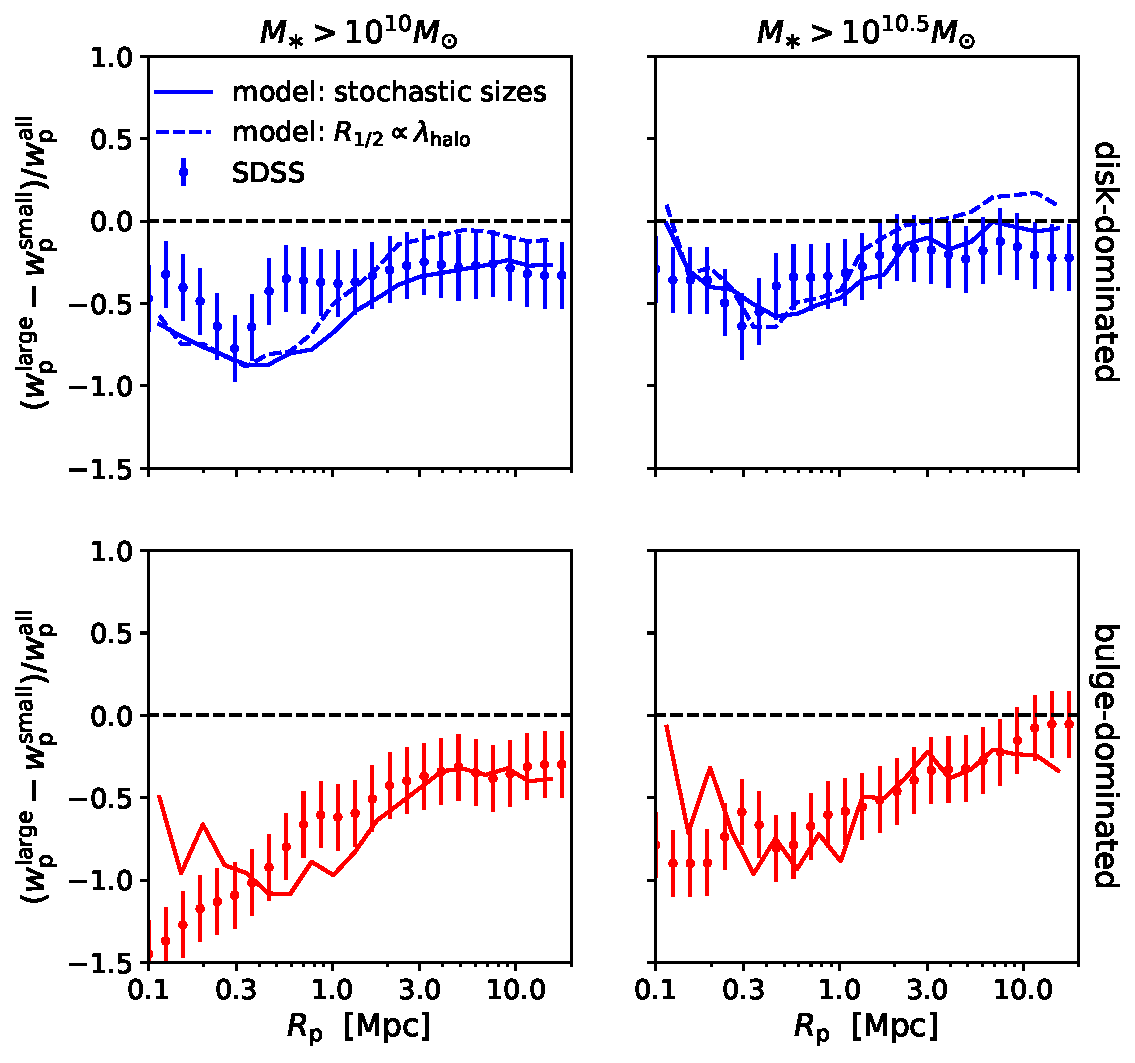
\includegraphics[width=8cm]{FIGS/size_clustering_ratios_bt_decomposition_spin_size_correlation.pdf}
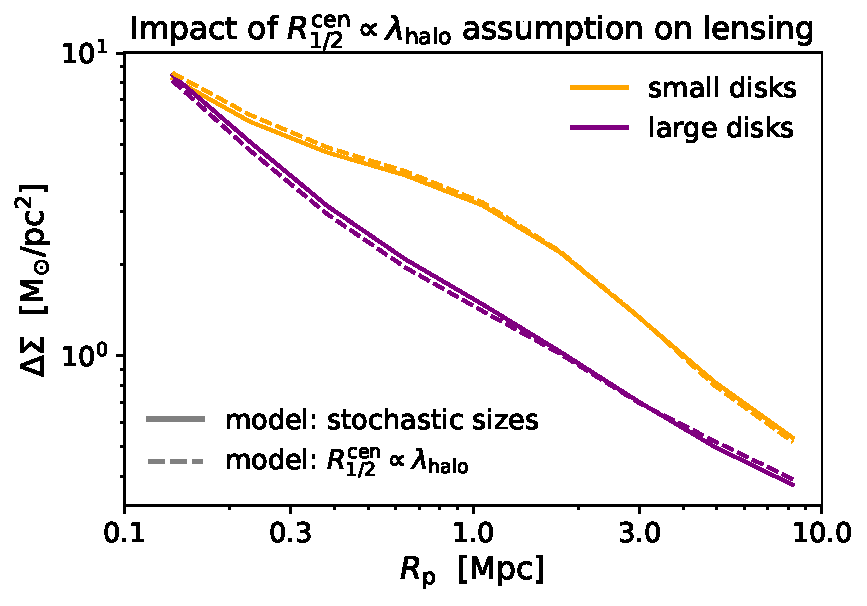
\includegraphics[width=8cm]{FIGS/central_lensing_spin_size_correlation.pdf}
\caption{
{\bf Clustering and lensing provide no constraining power on the assumption that $\rhalfdisk\propto\halospin.$}
We compare the predictions between our fiducial model in which sizes are purely stochastic, and an alternative model motivated by \citet{mo_mao_white98} in which central galaxy disk size is maximally correlated with host halo spin at fixed stellar mass \citep[implemented via conditional abundance matching, e.g.,][]{hearin_etal13b}. The tiny differences between the solid and dashed curves imply that conventional large-scale structure measurements cannot even in principle provide compelling evidence pertaining to the assumption that $\rhalfdisk\propto\halospin.$
}
\label{fig:halospin_lensing}
\end{figure}
%-----------------------------------------------------------------------------------------------------

The top panel of Figure \ref{fig:halospin_lensing} shows a comparison of the $\rhalf$ clustering ratios of our fiducial model to the alternative CAM model in which $\rhalfdisk\propto\halospin.$ Evidently, for galaxies in this stellar mass range, the strength of $\halospin$ correlations with the cosmic web are sufficiently weak as to produce almost no measurable impact on the $\rhalf-$dependence of the clustering of disk-dominated systems.

Of course it is possible that galaxy clustering is poorly suited to detect $\rhalfdisk-\halospin$ correlations, which instead manifest in some alternative measurement of large-scale structure. For example, numerous studies of the $\halospin-$dependence of halo assembly bias have shown that low-spin halos are preferentially found in environments of below-average dark matter density relative to high-spin halos of comparable mass \citep[see, for example,][]{lee_etal17}.

Motivated by these results, we show in the bottom panel of Fig.~\ref{fig:halospin_lensing} an idealized mock measurement of the lensing of central galaxies identified with perfect fidelity. Solid curves show $\Delta\Sigma$ signal of our fiducial model centrals, dashed curves the alternative CAM model. Again we see that $\rhalfdisk-\halospin$ correlations are simply not strong enough in $L_\ast$ galaxies to produce a compelling signal. These results imply that it will be extremely challenging to either confirm or refute the $\rhalfdisk\propto\halospin$ hypothesis using large-scale structure measurements. We discuss this further in \S\ref{subsec:mo_status}.


\section{Discussion}
\label{sec:discussion}


\subsection{Implications for Satellites}
\label{subsec:satellite_discussion}

\subsection{State of the $\rhalfdisk\propto\halospin$ Hypothesis}
\label{subsec:mo_status}

\subsection{Progression from Backwards to Forwards Modeling}
\label{subsec:forwardsmodeling}

\subsection{Relation to Previous Work}
\label{subsec:previouswork}

\subsection{Future Directions for Empirical Modeling of Morphology}
\label{subsec:future}


\section{Conclusion}
\label{sec:conclusion}

\subsection{Summary}
\label{subsec:summary}

\section*{Acknowledgments}

APH thanks John Baker for the {\em Toejam \& Earl} soundtrack. 

\bibliography{galsize_paper}

\end{document}







